\documentclass[]{article}
\usepackage{graphicx}
\graphicspath{ {./images/} }
\usepackage{hyperref}

\hypersetup{
	colorlinks=true,
	linkcolor=blue,     
	urlcolor=blue
}

%opening
\title{CSCI 337 - Note-taking app - Final Report}
\author{Logan Humbert}

\begin{document}
	
	\maketitle
	
	\pagebreak
	
	\tableofcontents
	
	\listoffigures
	
	\pagebreak
	
	\section{Description of the application}
	
	This little mobile application aims to let students taking notes for their different classes, and organizing them by class.
	
	\section{Requirements}
	
	\begin{itemize}
		\item \textbf{Who are the users? } The users are students (College, High School, Middle School, ...)
		
		\item \textbf{Who are the customers?} This app is only made in a school context. There is no real customer for it.
		
		\item  \textbf{User stories:}
			\begin{itemize}
				\item As a new user, I want to add my different classes, and start adding notes for them
				
				\item  As a regular user, I keep adding a new note during a lecture in my different classes, then I review them when I study.
				I can easily modify the content of the note if I need to.
			\end{itemize}
		
	\end{itemize}
	
	\section{Features}
	
	The user should be able to complete these different tasks easily:
	
	\begin{itemize}
		\item See his different classes
		\item Add/edit or delete a class
		\item Create/edit/delete a note for any class he has created
		\item View a note
		\item  Search for a class or a note by typing a part of its name
	\end{itemize}
	
	\pagebreak
	
	\section{Iterative design}
	
	\subsection{Sketches on paper}
	
	Here is a first sketch of the different pages of the app, and the transitions between them:
	
	\begin{figure}[!htb]
		\centering
		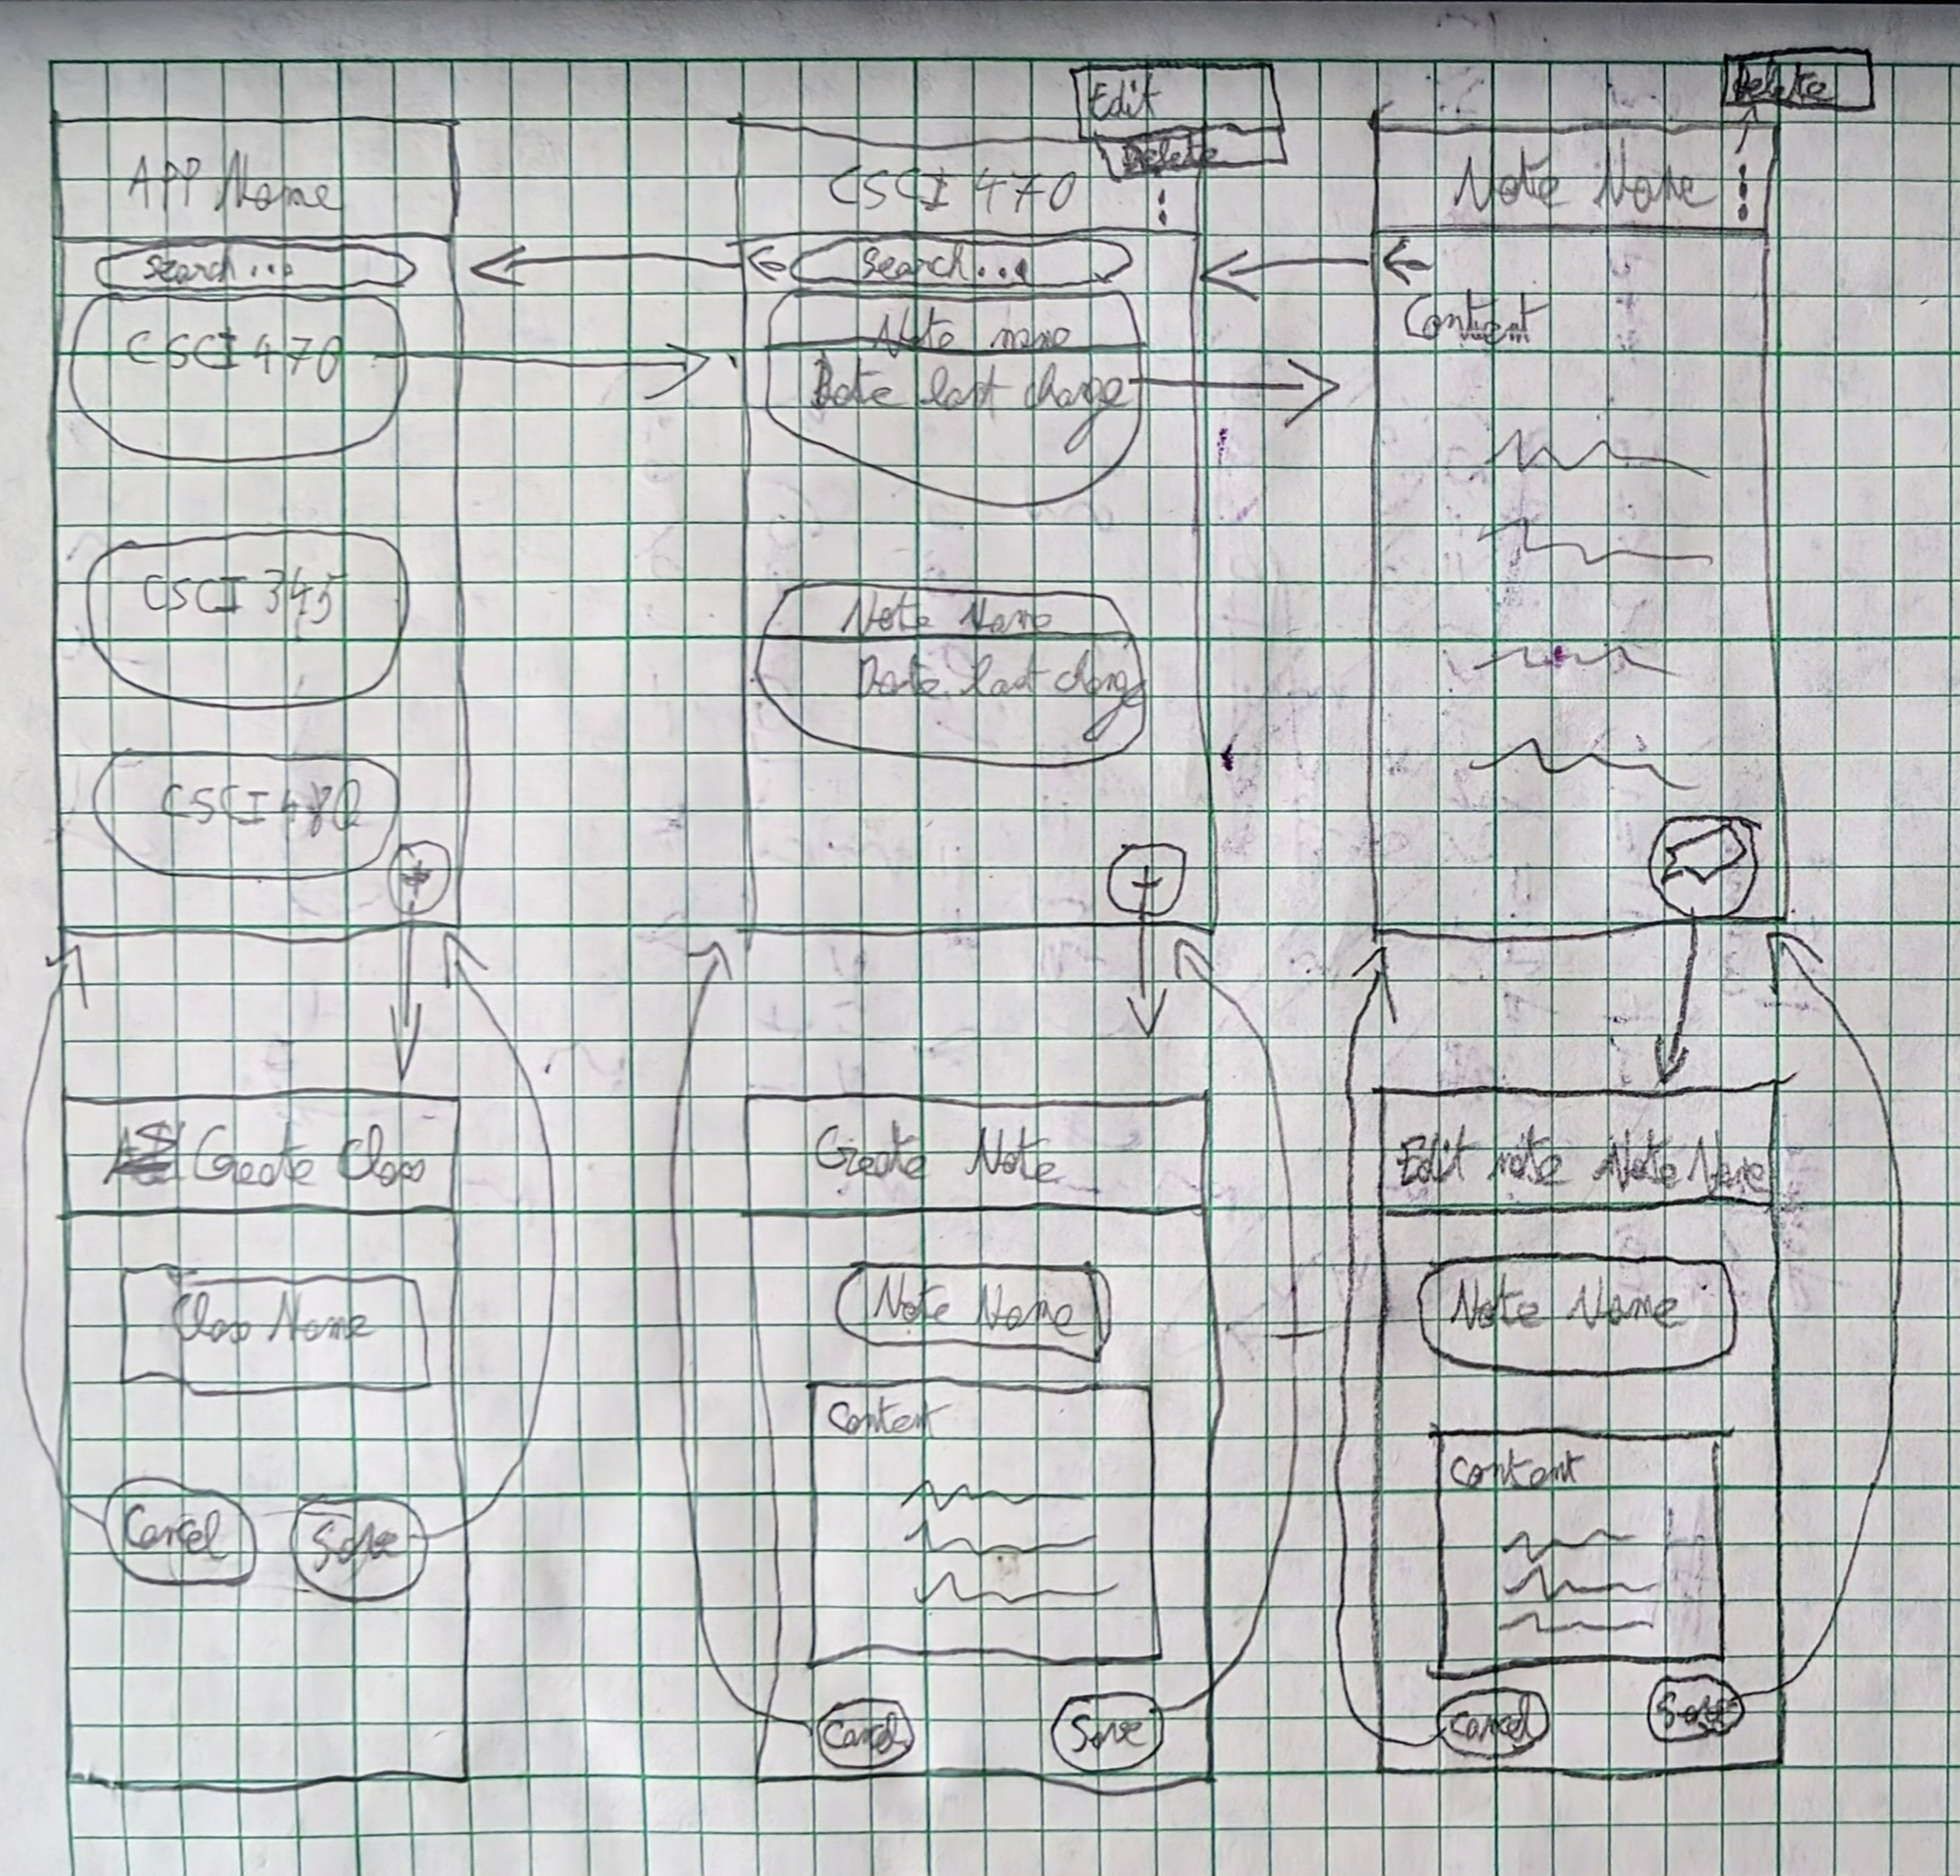
\includegraphics[scale=0.1]{first_sketch}
		\caption{First sketch on paper}
	\end{figure}
	
	I imagine having 5 different screens:
	
	\begin{itemize}
		\item The home page, containing a list of the existing classes.
		\item The add/edit class form
		\item The list of notes in a class
		\item The add/edit note form
		\item The content of a note
	\end{itemize}
	
	All pages can be accessed by clicking on a specific element, as the arrows on the sketches show.
	
	\pagebreak
	
	\subsection{Designing and prototyping on Figma}
	
	After drawing my first sketches on paper, I started making a more accurate and clean design of the UI on Figma, and I used its prototyping features to create the transitions between the pages of the app.
	
	For developing my app I decided to use Flutter, as I will explain more in details in the next section.
	As this framework uses the Google Material's design, I used their official figma template, which contains reusable Material component, so my Figma design could be as close as possible as the UI the final app will have.
	
	
	You can access my figma design \href{https://www.figma.com/file/ZOlxVGHb9fLdk5uUODqMU9/CSCI-337---Notes-Taking-App?type=design&node-id=54810%3A34721&mode=design&t=fS6KJvRgsvtgz9cf-1}{here}.
	
	I started by making the User Story "Create a class"
	
		\begin{figure}[!htb]
		\centering
		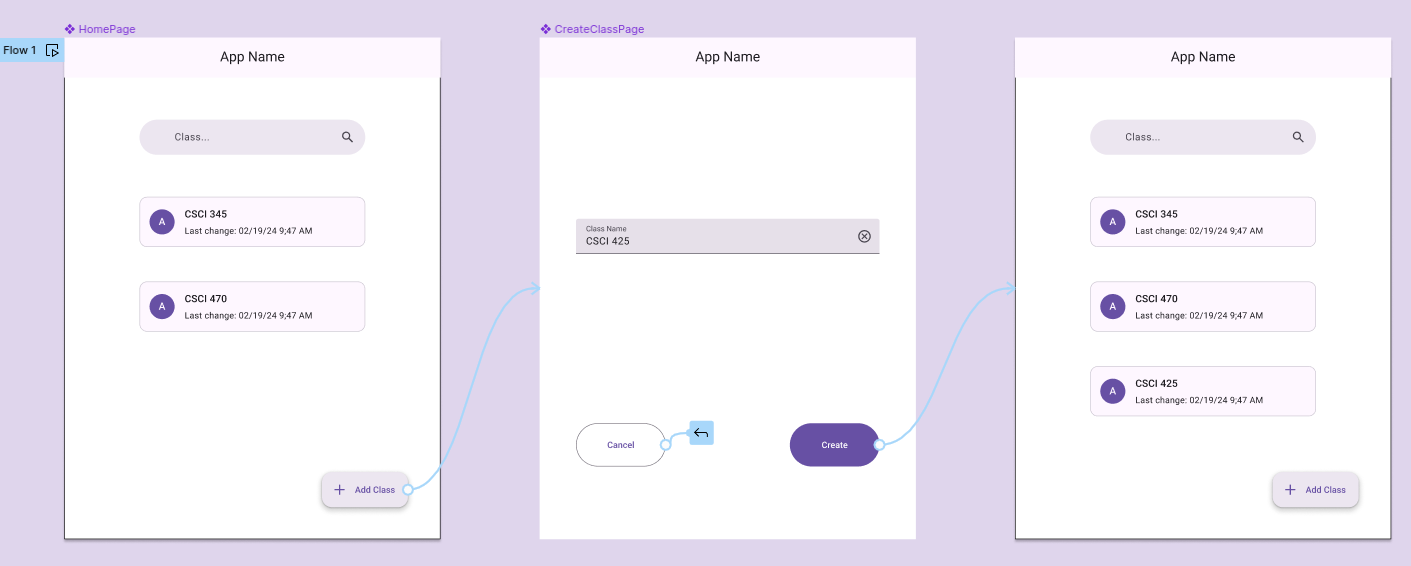
\includegraphics[scale=0.3]{figma_user_story_create_class}
		\caption{User story "Create Class" on Figma}
	\end{figure}
	
	From the home page that contains the list of our classes, a button lets the user create a class by giving it a name. It is then immediately available from the home page.
	
	\pagebreak
	
	Then I added the other user stories and added transitions between the different pages of the app:
	
	\begin{figure}[!htb]
		\centering
		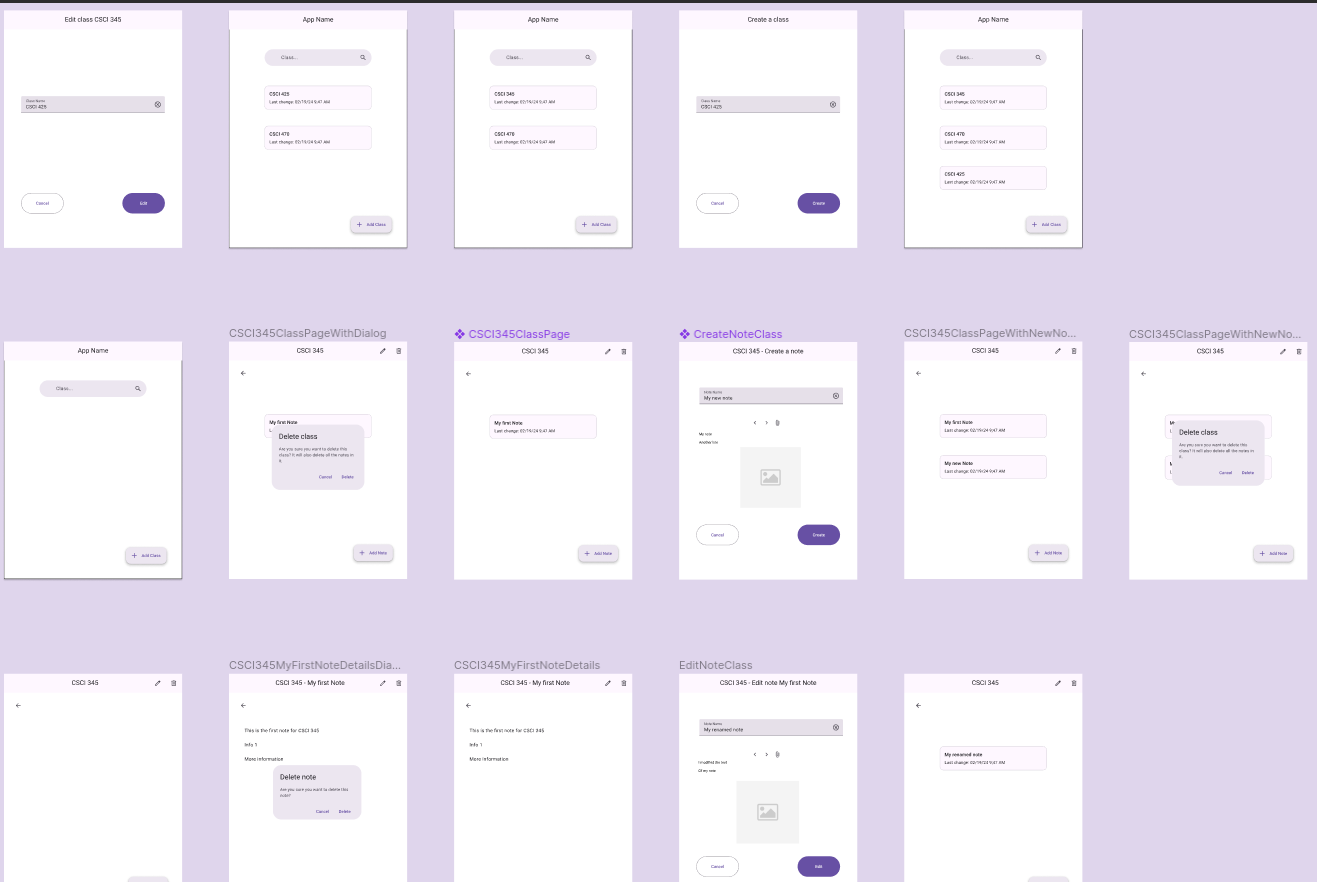
\includegraphics[scale=0.3]{figma_user_stories_finish}
		\caption{All user stories on Figma}
	\end{figure}
	
	Some pages of the app have been duplicated, as they simulate a change in database, or they display an additional graphical element, such as a dialog box, which is not possible to achieve directly on Figma.\linebreak
	These are used to obtain a better experience when we execute the prototype on figma.
	
	\pagebreak
	
	\subsection{Development with Flutter}
	
	After obtaining a first satisfying design and prototyping my app on figma, I started to develop my app.\linebreak
	
	I decided to use Flutter, which is an open-source framework created and maintained by Google.
	Its main advantage is that it allows building natively compiled multi-platform applications from a single codebase.\linebreak
	
	I focused mainly on making a web version as it is one of the easiest versions to debug, and it would allow my app to be available on any platform that has a web browser, such as windows and mac computers, Android and IOS phones and tablets.\linebreak
	
	Anyway, it would be very easy to build a native Android or IOS app for example, with none or just a few modifications of the code needed.\linebreak
	
	The source code and the instructions to build and run the Flutter app are available \href{https://github.com/Logan-Developer/ui-lahumbert/tree/main/FinalProject/note_taking_app}{here.}
	
	\subsection{Publishing the app}
	
	After judging that my app was complete and stable enough I decided to publish it.\linebreak
	For this I used a service named Github pages, that allows any Github repository to be accessed as a website.\linebreak
	The only cons of it is that it we cannot serve a nodeJS, apache or nginx server for example with this service.\linebreak
	As Flutter apps are don't require any of these, Github pages is a good choice.\linebreak
	
	The latest public version of my app is available \href{https://class-snap.tech/}{here.}
	
	\pagebreak
	
	\subsection{UI/UX tests}
	
	After developing and publishing my app I decided to do UI/UX tests.\linebreak
	For this, I asked other students, who were potential future users of my app to try it and give me feedback on the things they liked/disliked about the app, and reports of bugs.\linebreak
	
	Thanks to this useful information, I have been for example able to improve both the view that lists classes and the view that lists notes in a class.
	
	\begin{figure}[!htb]
		\centering
		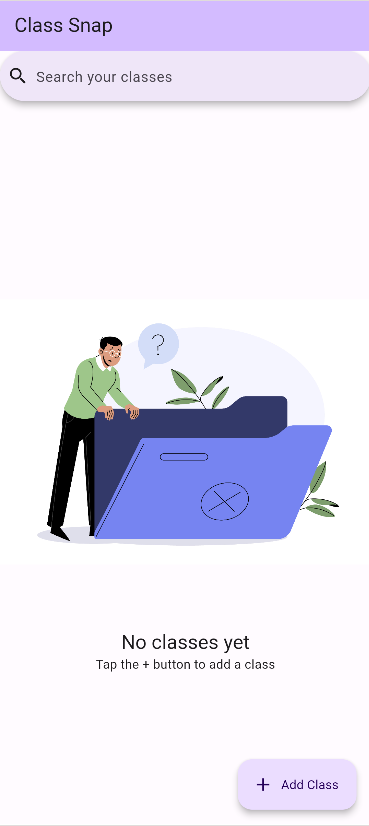
\includegraphics[scale=0.4]{ui_improve_class_list}
		\caption{Home page with empty list of classes}
	\end{figure}
	
	The graphics and text on the screenshot above displayed whenever no class has been created yet, were not present at first.\linebreak
	Therefor, some users did not know what to do and did not necessarily see the "Add Class" button in the lower right corner of the page.\linebreak
	Running UI/UX tests helped me being aware of the issue and addressing it.
	
	\pagebreak
	
	If these tests helped me improving some aspects of the app, they also helped me detecting bugs I did not noticed while I was developing the app and fixing them.\linebreak
	
	For example, if we named a class or a note with a '/' in it and we tried to access it, the application threw an error. This is because this special character is used in the routes leading to a class or a note, so the route was invalid in this specific case.
	
	\pagebreak
	
	\section{Conclusion}
	
	The development of this note-taking application employed an iterative design approach to create a user-friendly tool for students.\linebreak
	
	From initial paper sketches to Figma prototyping and ultimately a Flutter-based web application and then UI/UX tests, this project has let me exploring different important aspects of the creation of applications.\linebreak
	
	I have been able to respect the different requirements I have set for the app and to implement the different features features I wanted to have at first.\linebreak
	
	Future development could explore additional features like:
	
	\begin{itemize}
		\item Add more useful features such as the possibility of adding hand-drawn notes
		\item Add cloud storage support (for example via Firebase which has a great compatibility with Flutter)
		\item Add support for exporting notes such as pdf or word document
	\end{itemize}
	
	\pagebreak
	
	\section{Links}
	
	Here are the links to important resources:
	
	\begin{itemize}
		\item \href{https://github.com/Logan-Developer/ui-lahumbert/tree/main/FinalProject}{Project's repository} 
		
		\item \href{https://www.figma.com/file/ZOlxVGHb9fLdk5uUODqMU9/CSCI-337---Notes-Taking-App?type=design&node-id=54810%3A34721&mode=design&t=fS6KJvRgsvtgz9cf-1}{Figma Design}
		
		\item
		\href{https://class-snap.tech/}{Web version of the app}
	\end{itemize}
	
	\label{LastPage}
\end{document}